\section{Case Study: ThingSat}
\label{sec:case-study}

The ThingSat project~\cite{git:thingsat-repo} aims to benchmark ground-space
LoRa links on different frequency bands and demonstrate the
effectiveness of that technology inside a LEO (Low Earth Orbit) CubeSat.

ThingSat is deployed as a hosted payload on a shared 3U CubeSat:
\href{https://space.skyrocket.de/doc_sdat/stork-1.htm}{STORK-1} from the polish
start-up \href{https://www.satrevolution.com/}{SatRevolution}. The CubeSat was
launched on January 13th, 2022,currently in orbit at an altitude of 525 km (see its
\href{https://www.n2yo.com/database/?q=STORK-1\#results}{Two-Line Elements}).

The ThingSat payload now in orbit is used for Ocean level monitoring. However,
its design can be adequate for a wider variety of use cases, in Earth science
academic research (e.g. tacking the  melting of glaciers, pirate fishing...)
and in the industry for companies using geographically dispersed devices (e.g.
monitoring of tank ships...).

\begin{figure}[t]
\centering
    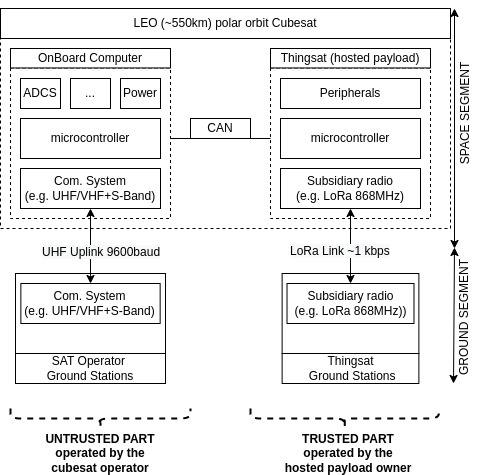
\includegraphics[width=0.35\textwidth]{Figures/globecom-thingsat-mods.jpg}
    \caption{ThingSat hosted payload: deployed components and architecture.}
    \label{fig:thingsat-archi}
\end{figure}

\subsection{Distributed System Architecture}
\label{sec:thingsat-hw}
\autoref{fig:thingsat-archi} describes the ThingSat deployment components, it gives an
overview of a typical CubeSat ecosystem, whereby the interaction with this payload
traverses untrusted elements.

\subsection*{Low-power Space Segment}
The Space Segment comprises the on-board computer (OBC) and hosted payloads, whom,
interconnected via a CAN bus, which share resources on the CubeSat.
\begin{itemize}
\item The OBC provided by the satellite operator consists on
a microcontroller with all its subsystems to operate the CubeSat:
Attitude Determination and Control System (ADCS),
communication subsystems (UHF/VHF/S-band for uplink/downlink and antennas) and
power subsystem (Battery Management, Energy Harvesting with Solar Panels, Auxiliary Power Supply).

\item We designed the ThingSat payload, using a STM32F405RG %STM32F446RE
microcontroller featuring an ARM Cortex-M4 core
and open source firmware based on RIOT~\cite{baccelli2018riot}. The ThingSat payload embeds both a
\href{https://www.semtech.com/products/wireless-rf/lora-gateways/sx1302}{Semtech SX1302 transceiver} for
communications on the 863\-870 MHz band and a \href{https://www.semtech.com/products/wireless-rf/24-ghz-transceivers/sx1280}{Semtech SX1280 transceiver}
for communications on the 2400\-2500 MHz band. Furthermore we designed a corresponding dual-band patch antenna (868MHz, 2.4GHz).
When active and using the 863\-870 MHz band, the ThingSat payload consumes at 3.3V:
(i) 90 mA in standby,
(ii) 110 mA during a frame reception (RX) and
(iii) 300 mA during a frame transmission (TX) at 27 dBm.
\end{itemize}

\subsection*{Ground Segments}
Ground Segment elements that communicate with the ThingSat payload are:
\begin{itemize}
\item \textbf{SatRevolution Ground Stations}: provided by the CubeSat operator \footnote{not
necessarily owned by the CubeSat operator} to communicate via UHF/VHF with the OBC,
and indirectly with the payload. This can be done directly od through a Command \&
Control Center, which acts as a broker between payload maintainers and hosted payload
(indirect access).
\item \href{https://github.com/thingsat/tinygs_2g4station}{\textbf{ThingSat LoRa Ground Stations}}:
that we designed, deployed and maintain, which can communicate via LoRa \textbf{directly} with the
ThingSat payload. These stations are based on an ESP32 microcontroller, and a 2.4GHz SX1280-LoRa
transceiver, also running an open source firmware based on RIOT.
\end{itemize}

\subsection{Communication Characteristics Overview}
\label{sec:thingsat-comm-characteristics}

ThingSat payload communicates either directly via low-power WAN, or indirectly
via the UHF/VHF link provided by the CubeSat's OBC.

\paragraph*{Direct communication patterns via low-power WAN}
ThingSat can communicate directly with LoRa. In principle, although it is not used as
such so far, this communication link could also be used to transport software updates.
As shown in \autoref{fig:thingsat-comm} the ThingSat payload may act as either:
(i) a Sat-IoT end-device (ED) that will send LoRa frames to terrestrial LoRaWAN gateways or ThingSat ground stations (GS), or
(ii) an in-orbit LoRa sniffer, or
(iii) a store-carry-and-forward LoRa gateway.

Patterns (i) and (ii) allow to benchmark simple ground-space LoRa links by
computing statistics over multiple sent/received frames.
Pattern (iii) is a more
complex scenario: the satellite stores packets received from GS/ED and deliver
them once GS/ED destinations are inside the footprint of the satellite.

\paragraph*{Indirect communication characteristics via UHF/VHF}
CubeSat-GS communications are typically done on amateur frequency
bands (UHF/VHF) with typically low data rates ranging from 9.6kbps to
100kbps.
A polar LEO satellite will typically pass over a given ground station 2 to 4 times/day,
each pass having a communication window of to 10 minutes.

For ThingSat, the CubeSat Operator provides only 2 ground stations (both in Europe), communicating with
the CubeSat via a 10-kbps UHF/VHF link. Thus, the daily throughput is roughly
1500KB (corresponding to 2 GS x 2 passes/day x 5-min pass duration x 10Kbps).
However, this throughput must be shared between communications to/from the OBC
(for telecommand/telemetry/update) and to/from hosted payloads. Therefore in practice,
the total communication budget available for ThingSat via the UHF/VHF link is around
300KB/day.

\paragraph*{Intermittent communication/power supply}
Last but not least, the ThingSat payload is not constantly powered on. Typically, at point any time,
only a single hosted payload is powered on. For a 3U, 1U is dedicated to the OBC
and the remaining 2U, available for hosted payloads (8 payloads slots of 0.25U
in the case of ThingSat). Therefore, on average ThingSat is powered only 1/8th (12.5\%) of the time
(modulo other factors such as mission specificities, regulations, battery level etc.).

\subsection{Hosted Payload Software Updates Requirements}
\label{sec:thingsat-update-req}
Data exchanges between the Payload Maintainer and ThingSat consist on
\textbf{downlinks}: used by ThingSat to send mission results (radio metadata, frame stats, collected LoRa frames)
and diagnosis data (debug info on failed missions/updates)l \textbf{uplinks}: used for software updates of two categories:
\begin{enumerate}
    \item Firmware updates: to fix bugs, add/improve functionality (typically $\sim 200kB$ per FW, 1 FW/month);
    \item Mission updates: to configure scenarios (typically $\sim 700B$ per mission scenario, 1 scenario/day);
\end{enumerate}

\begin{figure}[t]
    \centering
    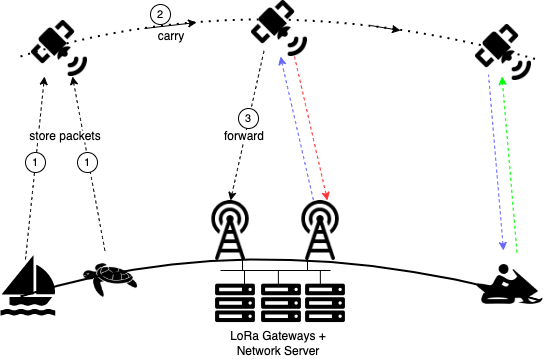
\includegraphics[width=0.4\textwidth]{Figures/thingsat-dtn.png}
    \caption{ThingSat in-orbit communication patterns.}
    \label{fig:thingsat-comm}
\end{figure}
